\chapter{Redox: Pathway Exploration}
\label{chap:redox}

\section{Purpose}
The purpose of this chapter is to describe Redox, a web application designed to run offline or deployed online, that is used to visualize, explore, and analyze large sets of biochemical network pathways.
Redox was developed with the scientists at Arzeda Inc (\url{http://arzeda.com/}) as the primary end users and source of feedback.
However, Redox is an example of modular design using the yeoman build tools.
Additional data controllers and templates may also be easily added to extend compatibility with input sources and custom layouts.

\section{Motivation}
\subsection{Metabolic engineering of microorganisms may yield new ways of producing valuable commodities}
\subsection{The space of candidate pathways is extremely large}
KEGG
Biochemical reactions 9,647
Metabolites and other small molecules 17,257
\subsection{Semi-automated pathway selection requires user curation}


\section{Solution}
\subsection{Visualize candidate pathways}
\subsection{Sorting, filtering, and pinning to hone in on desired output}
\subsection{Export curated selection of pathways}

\begin{figure}
  \centering
  \begin{subfigure}[b]{\textwidth}
    \includegraphics[width=\textwidth, page=5,trim=0.37cm 3.65cm 13.1cm 3.3cm, clip=true]{images/Figures.pdf}
    \caption{The table view lists all pathways in a paginated format.
      The user can browse the tabulated pathways and sort by metadata.}
    \label{Figure:redox-table-view}
  \end{subfigure}
  \begin{subfigure}[b]{\textwidth}
    \includegraphics[width=\textwidth, page=5,trim=13.1cm 3.65cm 0.37cm 3.3cm, clip=true]{images/Figures.pdf}
    \caption{Pinned pathways are added to the side bar and encoded with a color from palette.}
    \label{Figure:redox-table-pinned}
  \end{subfigure}
  \caption{The Redox Table View allows users to parse through numerous pathways and select individual candidates for further examination.}
  \label{Figure:redox-table}
\end{figure}

\begin{figure}
  \centering
  \begin{subfigure}[b]{\textwidth}
    \includegraphics[width=\textwidth, page=6,trim=0.37cm 3.65cm 13.1cm 3.3cm, clip=true]{images/Figures.pdf}
    \caption{Mouse hover over the pathway list color codes all the related reactions and species involved in the pathway. In this template, circles indicate species and squares denote reactions.}
    \label{Figure:redox-graph-highlight1}
  \end{subfigure}
  \begin{subfigure}[b]{\textwidth}
    \includegraphics[width=\textwidth, page=6,trim=13.1cm 3.65cm 0.37cm 3.3cm, clip=true]{images/Figures.pdf}
    \caption{Hovering over the next list item will quickly switch the color coding, allowing the user to explore the pathways.}
    \label{Figure:redox-graph-highlight2}
  \end{subfigure}
  \caption{Redox Graph creates a connected network diagram from all selected pathways.}
  \label{Figure:redox-graph-highlight}
\end{figure}

\begin{figure}
  \centering
  \begin{subfigure}[b]{\textwidth}
    \includegraphics[width=\textwidth, page=7,trim=0.37cm 3.65cm 13.1cm 3.3cm, clip=true]{images/Figures.pdf}
    \caption{In the sidebar, sliders allow the user to interactively change force directed layout settings, such particle charge and gravity.}
    \label{Figure:redox-template-a}
  \end{subfigure}
  \begin{subfigure}[b]{\textwidth}
    \includegraphics[width=\textwidth, page=7,trim=13.1cm 3.65cm 0.37cm 3.3cm, clip=true]{images/Figures.pdf}
    \caption{Graphene templates may be swapped out on the fly to change the graph.
      Due to the separation of model and view, the underlying data is unchanged when the view is switched.}
    \label{Figure:redox-template-b}
  \end{subfigure}
  \caption{The Redox layout is highly customizable.}
  \label{Figure:redox-template}
\end{figure}

\begin{figure}
  \centering
  \begin{subfigure}[b]{\textwidth}
    \includegraphics[width=\textwidth, page=8,trim=0.37cm 3.65cm 13.1cm 3.3cm, clip=true]{images/Figures.pdf}
    \caption{Upon node hover, a pop-up window shows the relevant chemical structure of the species of reaction diagram.
      The sidebar also populates with a link to the ChEBI web page.}
    \label{Figure:redox-detail-hover}
  \end{subfigure}
  \begin{subfigure}[b]{\textwidth}
    \includegraphics[width=\textwidth, page=8,trim=13.1cm 3.65cm 0.37cm 3.3cm, clip=true]{images/Figures.pdf}
    \caption{Clicking on the link to ChEBI leads directly to the species information page.}
    \label{Figure:redox-detail-chebi}
  \end{subfigure}
  \caption{Exploring graph details.}
  \label{Figure:redox-detail}
\end{figure}

\section{Implementation}
\subsection{Data and layout controllers in Graphene}
\subsubsection{Data model}
\subsubsection{Separation of concerns}
\subsubsection{Sorting and filtering}
\subsection{Swappable layout templates}
\subsection{Integration with web interface}

\section{Future Directions}
